\documentclass{article}

\usepackage[margin=1in]{geometry}
\usepackage{amsmath}
\usepackage{graphicx}

% Redefining maketitle to adjust the title font size
\makeatletter
\renewcommand{\maketitle}{\bgroup\setlength{\parindent}{0pt}
\begin{flushleft}
  \textbf{\LARGE \@title} \\ % Change \LARGE to desired size if needed
  \vspace{0.5em}
  \@author
\end{flushleft}\egroup
}
\makeatother

\title{JiaShua - A Complex System Simulation: A Report}
\author{Nan Jia, Joshua Rollins}

\begin{document}
\maketitle
\section*{Abstract}
This report demonstrates the design and simulation of a call center with various random variables that affect the system. The report will show the planning, design, structure, and simulation of the system along with the results of the simulation pertaining to its original variables and setup then our recommendations to meet the manager’s desired performance requirements.

\section{Introduction}
This mid-term project is to simulate a call center mechanism, originally containing two queues, one for callers asking about car-stereos and one for other products. The call center is a complex system with multiple variable types. Those include server and queue statuses, event calendar, global variables for tracking and measuring performance, and random variables. Those elements aim to mimic a real-life call center scenario and to provide a way to measure the performance of the call center. The programming language used is \emph{Python}. This report consists of the following sections containing sections (1)-(10) of the project requirements: system description (1-4), simulation method (5-7), simulation result (8), and conclusion (9-10).

\section{System Description}
A major auto retailer's call center is examined for its call processing, especially during midday peak times in the upcoming holiday season. When customers call, they connect to a switch. If more than ten calls are on hold, the customer receives a busy tone and hangs up. If not, the call proceeds to an interactive voice response (IVR) unit where callers choose between car-stereo products or other products. The call is then queued according to the product type until a sales representative is available. The goal is to determine the minimum number of sales representatives required to ensure less than 2\% of calls wait more than 1 minute and less than 3% are refused at the switch.

Key assumptions include the instantaneous action of the switch and the IVR unit's capacity to handle multiple calls simultaneously. The IVR involves a pure delay, which must be accounted for. The project employs a physical random number generator using two dice (DICE). This DICE determines various delays and product type requests. For instance, the time between call arrivals is calculated as (DICE * 0.333) minutes. The IVR unit's delay is (DICE * 0.3) minutes, while car-stereo and other product processing times are (DICE * 2) minutes and (DICE) minutes respectively. Lastly, if the DICE rolls a value less than or equal to 4, it's set that the call is for a car stereo, representing an average 16.7\% of all calls. Otherwise, it's for other products. \\

\par
1. Identify state variables; \\ 
System clock (measured in minutes) \\
Number of callers currently in the IVR relay system \\
Number of callers in the other products queue \\
Number of callers in car-stereo queue \\
Car-stereo status - idle or busy based on if the server is currently attending to a customer \\
Other product status - idle or busy based on if the server is currently attending to a customer \\
Event calendar - A pandas DataFrame containing all the events to be ran by the simulation \\
Event history - A pandas DataFrame containing all the events which were run by the simulation. This should be full by the end of the simulation. \\

\par
2. Identify events and event-attributes; \\
Event 1: Arrival of a help request call from a caller, as specified from events calendar. \\
Event 2: Call splits to a sales representative’s queue from IVR unit. \\
Event 3: End of the call, when the sales representative finishes talking with the caller or the busy signal causes the call to hang up before entering the IVR unit. \\
Event 4: Call center closes at 4pm. \\
Event 5: End of the simulation.\\
\par
3. Identify random variables;

DICE: The results of two dice whose results are summed. This is rerolled for every random variable.
Time between arrivals of calls: (DICE * 0.333) minutes \\
IVR unit delay: (DICE * 0.3) minutes \\
Product type for the caller: DICE <= 4 \\
Car-stereo call processing: (DICE * 2) minutes \\
Other-product call processing: (DICE) minutes \\
\par
4. Identify global variables that are used to track and measure performance; \\
In lieu of individual global variables to track many metrics over simulations and iterations of simulations, we have used an event history DataFrame to track the performance. Measures of performance were taken from calculations from the event history, for example: Number delayed, total served customers, total waiting time, mean of waiting time, variance of waiting time, standard deviation of waiting time, 95% Confidence Interval of waiting time.



\section{Simulation Method}

5. Construct the random number generator, DICE
We constructed the random number generator, DICE, using the random integer generation function from python’s random package. Producing a number from 1 to 6 with a uniform distribution, we sum two independent rolls to get a normal distribution, as shown in the figure below containing a trial of the DICE function over 100,000 calls. \\
\par

6. Implement the simulation clock and the advance of the simulation clock, as well as an event calendar (event list) which is a list of events as they are scheduled. In every simulation, there is only one calendar and it is ordered by the earliest scheduled-time first. \\
\par

The event calendar is produced outside of the classes on a per-simulation basis. It is produced by generating arrivals spaced out from each other by DICE * 0.333 minutes until the business hours are complete. We implement a simulation clock within the state variables of the callCenter class. The clock is advanced by the events that are produced and delays which are calculated in the callCenter class. Further references can be found by searching “self.clock” within the main.py file. \\
\par
7. Construct control logic flow charts before you start coding the simulation program. \\

This section will present the big picture of the simulation as Figure~\ref{fig:call_center}. We start a loop within the main function. When we call this function, the server will be turned on. Then, the program will check whether it is $4$ pm because the business hours are from $11$ to $4$ that is $300$ minutes. If it is past business hours, the system will directly jump to Event 5: simulation termination. After checking the system's event calendar it will be ready to feed into the core functionality of this call center. \\
\par
First, the program will verify whether there is an available spot to serve the incoming customer as shown in Figure~\ref{fig:call_center}, the box of Busy Signal. If not, the customer will hang up. Otherwise, the customer will be served by the server. The server will check whether the customer is calling for car stereo or other products. If the customer is calling for a car stereo, the server will serve the customer for random minutes. After the server finishes serving the customer, the server will check whether there is a customer in the queue. If there is a customer in the queue, the server will serve the customer. Otherwise, this representative  will be set available. 
\begin{figure}[t!]
\centering
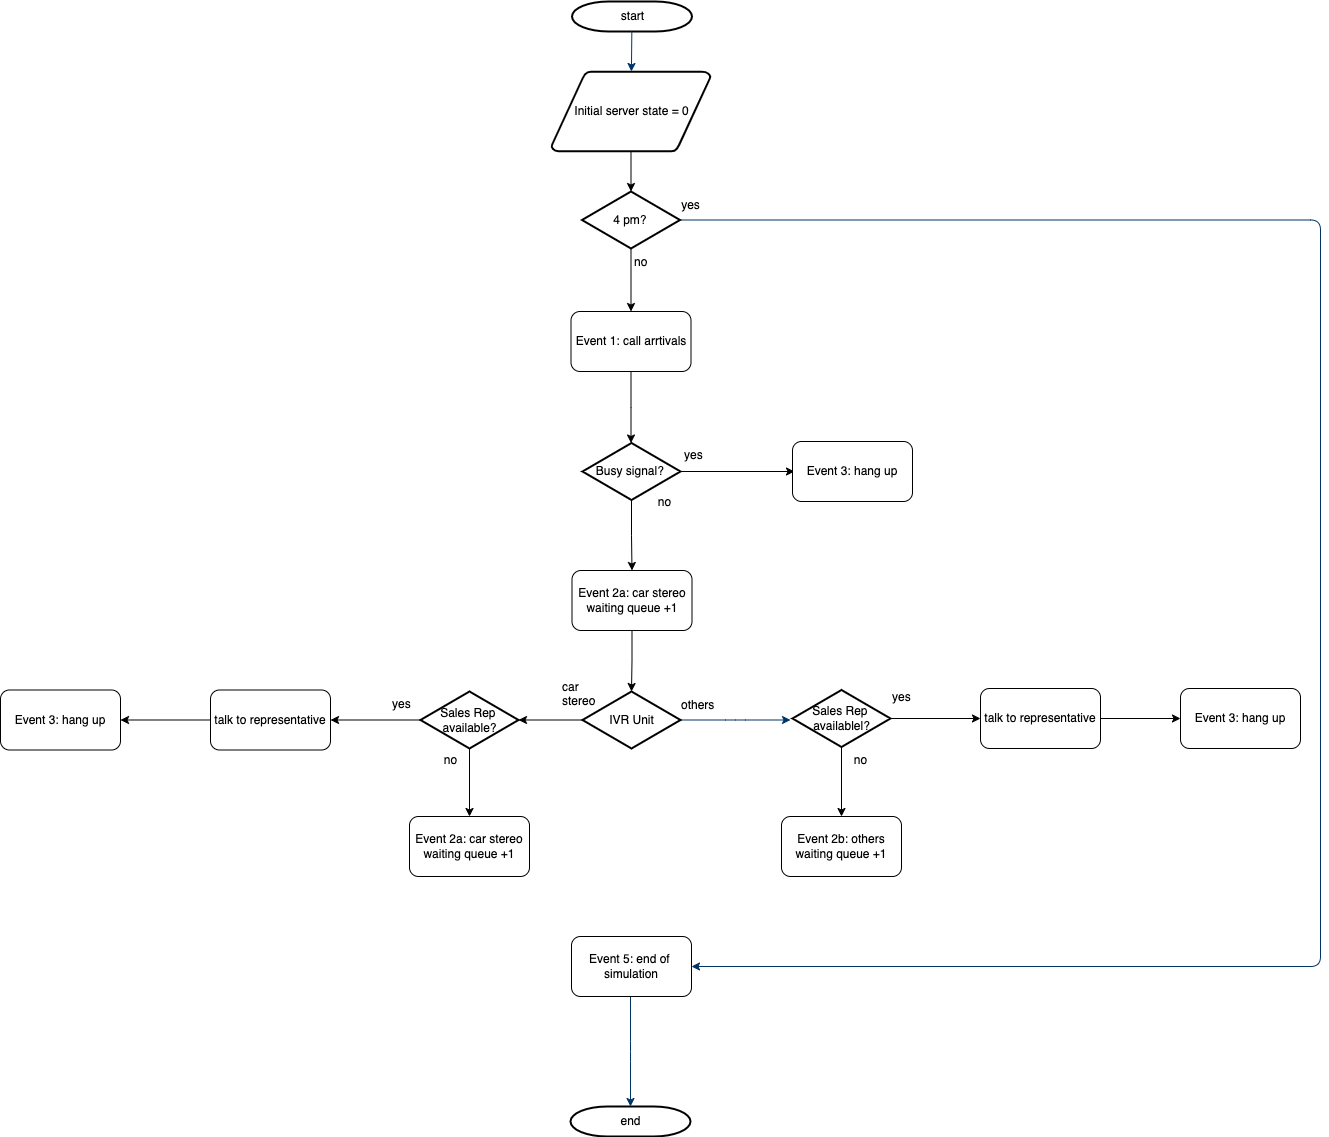
\includegraphics[width=1.1\textwidth]{call_center.png}
\caption{Call Center Control Flow Chart}
\label{fig:call_center}
\end{figure}

\section{Simulation Result}
8. Develop and run your simulation program with the given initial and end conditions:  Simulation start with “empty and idle” condition (no cars arrival yet, queues are empty and servers are idle).  Simulation runs for midday peak hours from 11am to 4pm, no break during operation.  You need to run the simulation multiple time (N=30 iterations or replications) to get statistical answers to the manager’s questions, as well as other key performance measures, (such as server utilization, maximum, average, minimum values of waiting time in each queue) in terms of means, standard deviation and a confident interval with 95% confidence. 


\section{Conclusion}
9. Provide your recommendations (alternatives) to the manager as of how to improve the system to meet the performance goals. Justify your recommendations by run simulation with your recommended system configurations. This is called what-if analysis. 10. One of the recommendations is “cross-training” were all representatives to process both call types, all calls could wait in a single queue for the next available representative. 


\end{document}
